\documentclass[xcolor={usenames,dvipsnames,svgnames}]{beamer}

\usetheme{mun}
\setbeamercovered{transparent}
\usepackage{multido}

\usepackage{biblatex}
\bibliography{\jobname}

\title{Text Summarization}
\subtitle{Computer Science 4750}
\author{Noah~Gallant\,~//~Jacob~House}
\date{Fall 2018}

\begin{document}
\begin{frame}[plain]
\titlepage
\end{frame}

\startheads

\section*{Outline}
\begin{frame}
	\tableofcontents
\end{frame}

\section{Topic}
\begin{frame}

\end{frame}

\section{Different Approaches}

\subsection{Evolutionary Algorithm}
\begin{frame}
%Different candidate summarizations are made and a score each of their fitnesses is computed. Those with the highest fitness move on to create new offspring candidates which share positive traits of both parents.
\begin{tabular}{ll}
	\begin{minipage}{0.6\linewidth}
		\begin{enumerate}
			\item Assign weights to text features
			\item Create population of distinct summaries
			\item Assess fitness
			\item Choose summaries with highest fitness
			\item Create offspring from chosen summaries
			\item Repeat steps 3--5 until the summary is concise enough
		\end{enumerate}
	\end{minipage}
	& \begin{tabular}{c}
		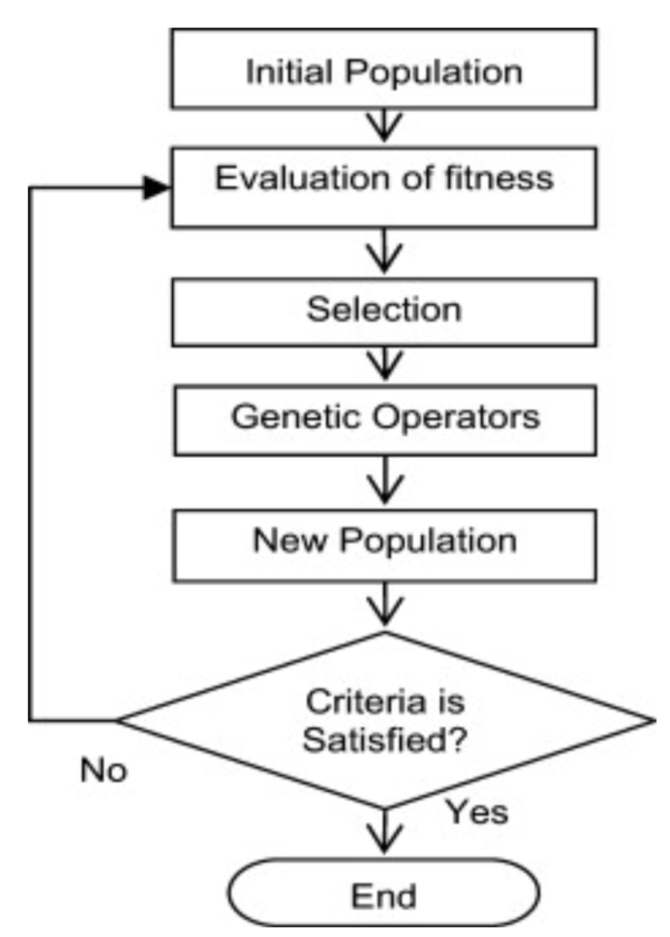
\includegraphics[width=0.3\linewidth]{ga}
	\end{tabular}
\end{tabular}
\end{frame}

\subsection{Nested Tree}
\begin{frame}
The goal in this approach is to repeatedly trim the tree until the desired summary size is reached.
\vskip 1pc
\begin{tabular}{ll}
\begin{minipage}{0.45\linewidth}
\begin{itemize}
	\item Tree structure is dependency based
	\begin{itemize}
		\item Inter-sentence
		\item Inter-word
	\end{itemize}
	\vskip 1pc
	\item Tree trimming to reduce size
	\begin{itemize}
		\item Removes duplicates
		\item Removes less important nodes
	\end{itemize}
\end{itemize}
\end{minipage}
& \begin{tabular}{c}
	\hskip -3pc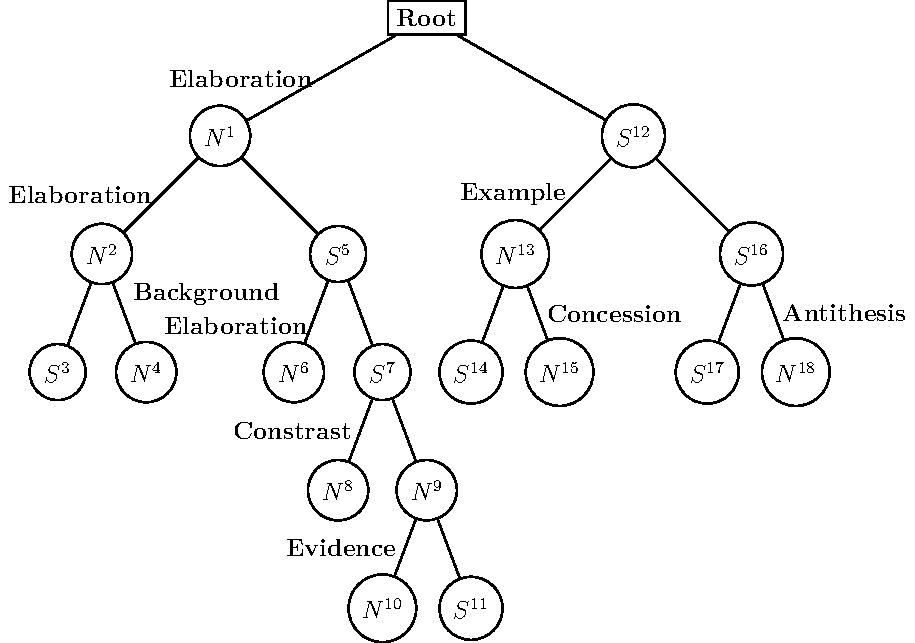
\includegraphics[width=0.6\linewidth]{tree}
\end{tabular}
\end{tabular}
\end{frame}

\subsection{Graph-Based}
\begin{frame}
\begin{itemize}
	\item Nodes created for each sentence
	\vskip 6pt
	\item Edges added between sentence nodes
	\vskip 0pt
	\begin{itemize}
		\item Adjacent sentences in the text
		\vskip 4pt
		\item Sentences that share common words
		\vskip 6pt
	\end{itemize}
	\item Edges with higher weight denote dependency
	\vskip 6pt
	\item Nodes (sentences) with highest total edge weight should be included in the summary
\end{itemize}
\end{frame}

\section{Our Design}
\multido{\i=1+1}{4}{%
\begin{frame}
	\centering
	\includegraphics[width=.75\linewidth]{venn-\i}
\end{frame}
}

\section{Implementation}
\subsection{The {\tt Graph} Class}
\begin{frame}
content...
\end{frame}
\subsection{The {\tt Node} Class}
\begin{frame}
content...
\end{frame}
\subsection{The {\tt Edge} Class}
\begin{frame}
content...
\end{frame}


\section{References}
\begin{frame}[allowframebreaks]
\nocite{*}
\printbibliography
\end{frame}
\end{document}